\documentclass[11pt]{article}
\usepackage{geometry,marginnote} % Pour passer au format A4
\geometry{hmargin=1cm, vmargin=1.5cm} % 

% Page et encodage
\usepackage[T1]{fontenc} % Use 8-bit encoding that has 256 glyphs
\usepackage[english,french]{babel} % Français et anglais
\usepackage[utf8]{inputenc} 

\usepackage{lmodern}
\usepackage[np]{numprint}
\setlength\parindent{0pt}

% Graphiques
\usepackage{graphicx,float,grffile}
\usepackage{tikz,pst-eucl,pst-plot,pstricks,pst-node,pstricks-add,pst-fun,pgfplots} 

% Maths et divers
\usepackage{amsmath,amsfonts,amssymb,amsthm,verbatim,scratch3}
\usepackage{multicol,enumitem,url,eurosym,gensymb,tabularx}

\DeclareUnicodeCharacter{20AC}{\euro}



% Sections
\usepackage{sectsty} % Allows customizing section commands
\allsectionsfont{\centering \normalfont\scshape}

% Tête et pied de page
\usepackage{fancyhdr} \pagestyle{fancy} \fancyhead{} \fancyfoot{}

%\fancyfoot[L]{Collège Faubert}
%\fancyfoot[C]{\thepage / 6}
%\fancyfoot[R]{Série Générale}

\renewcommand{\headrulewidth}{0pt} % Remove header underlines
%\renewcommand{\footrulewidth}{0pt} % Remove footer underlines

\newcommand{\horrule}[1]{\rule{\linewidth}{#1}} % Create horizontal rule command with 1 argument of height

\newcommand{\Pointilles}[1][3]{%
  \multido{}{#1}{\makebox[\linewidth]{\dotfill}\\[\parskip]
}}

\newtheorem{Definition}{Définition}

\usepackage{siunitx}
\sisetup{
    detect-all,
    output-decimal-marker={,},
    group-minimum-digits = 3,
    group-separator={~},
    number-unit-separator={~},
    inter-unit-product={~}
}

\setlength{\columnseprule}{1pt}


\begin{document}

\textbf{Ex1 - Calculer}

Les triangles sont rectangles. À l'aide du théorème de Pythagore, faire le tableau et trouver les longueurs manquantes. 

\begin{figure}[H]
  \centering
  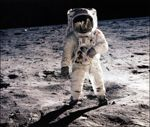
\includegraphics[width=0.4\linewidth]{4x1-pythagore/ex1.pdf}
\end{figure}

\Pointilles[5] 


\textbf{Ex2 - Égalité de Pythagore} - \textit{Écrire les égalités de Pythagore.}



\begin{multicols}{3}
Le triangle AZE est rectangle en A. \\ \Pointilles[1] \\
Le triangle QSD est rectangle en S. \\ \Pointilles[1] \\
Le triangle RTY est rectangle en Y. \\ \Pointilles[1] 
\end{multicols}


\textbf{Ex3 - Rédaction}

\begin{multicols}{2} \begin{enumerate}
  \item Le triangle UIO est rectangle en U. On a UI = 36cm et UO = 49cm. Calculer IO. \\ \Pointilles[7] \columnbreak
  \item Le triangle FGH est rectangle en G. On a GH = 54cm et GF = 78cm. Calculer FH. \\ \Pointilles[7]
\end{enumerate} \end{multicols} 


\begin{multicols}{2} 

\textbf{Ex4 - Problème} \\

Un pont à haubans relie un point A à un point B. Il est composé d'un mat de 28m de haut. et de haubans reliant le haut du mat aux extrémités du pont. Calculer la longueur totale des haubans. \columnbreak

\begin{figure}[H]
  \centering
  \includegraphics[width=0.7\linewidth]{4x1-pythagore/pb1.pdf}
\end{figure}

\end{multicols} 

\Pointilles[8]

\end{document}
